\chapter{Introduction}

Mother Nature has created a diverse set of awe-inspring motions in the animal kingdom: Birds can fly in the sky, fishes can swim in the water, geccos can crawl on vertical surfaces, and cats can reorient themselves in midair. These motions are elegant, agile, efficient, and more importantly, inspiring. Some of the best human innovations can be attibuted to the inspiration from locomotion of animals. For example, airplane, submarine and more recently, MIT cheetah and StickyBot, all can find deep roots from nature's design. Studying the motions designed by nature is not only a scientific quest that quenches our curiosity, but also an important step towards synthesizing them in a way that can fundamentally change our life.

The research of locomotions will have broad and impactful applications. One important application is entertainment. In movies and games, we need to faithfully reproduce the motions of animals on the screen. Moreover, we often need to create realistic animations for fantacy creatures that may not exist on our planet. The synthesized motions of these characters need to appear realistic. The applications of motion synthesis go far beyond just the entertainment industry. For example, it can enable us to build powerful robotic exoskeletons that help gait habilitation, assist paralyzed to walk and boost human power. In addition, motion synthesis can help us develop robotic systems with extensive flexibility, agility and maneuverability. These next-generation robots are expected to free human from dangerous missions in military, exploration and rescuing. 

Although we often take our locomotion ability for granted since we can perform them so effortlessly, motion synthesis is a notoriously difficult problem because locomotion involves sophisticated neuromuscular control, sensory information processing, motion planning, coordinated muscle activation, and complicated interactions between the body and its physical environment. It poses a grand challenge for scientists, engineers and artists. Despite extensive studies for centuries, we are still nowhere near fully understanding the underlying physics and control mechanisms that govern these motions. The focus of this dissertation is to present a set of powerful computational tools that facilitate the motion synthesis for locomotion of humans and animals, with the applications in character animation and robotics.

In the last few decades, we have seen tremendous advance in motion synthesis. Some of the most breathtaking movies, such as Harry Porter, Avatar and Life of Pi, rely heavily on computer generated character animations. Nowadays, it is almost impossible for the audience to tell apart the computer-synthesized motions from the real footage. In robotics, motion synthesis is also widely used to design agile and robust locomotion controllers. The MIT Cheetah can run up to 10 miles per hour and jump over obstacles. The Big Dog from Boston Dynamics can walk robustly in adversary environments, including icy or rocky terrains. The soft body robots can take advantage of their flexible bodies to navigate narrow and unstructured spaces. The humanoid robots, such as Petman and Asimo, was able to demonstrate a repertoire of locomotion skills, including walking, running, dancing and climbing stairs.

Behind these realistic animations and sophisticated robots lies countless hours of tedious manual work of highly-specialized experts. For example, to produce a 100-minute feature film at Pixar can take dozens of artists and engineers more than five years of development. In today's animation pipeline, the most popular techniques to synthesize motions are key frames or motion capture, both of which require artistic expertise and laborious manual work. Even worse, the knowledge and efforts that are put into one animation sequence are not necessarily generalizable to other motions. In my point of view, these are not efficient or principled ways of motion synthesis.

\textbf{A principled way is to develop computational tools, including physical simulations and optimization methods, to study the fundamental factors that have shaped our motions.} Our motions are shaped through millions of years of optimization (evolution) in a world that obey physical laws. This insight has motivated a new paradigm of \emph{simulation-driven controller optimization} in both character animation and robotics. The two key components of this paradigm are physical simulation and controller optimization. We first build a physical simulation to model the physical world and then perform optimization to control the motions of characters so that they can move more efficiently and robustly in the simulated environment. With these computational tools, natural movements, including walking \cite{}, running \cite{}, flying \cite{} and swimming \cite{} emerge automatically. In addition to these basic locomotion tasks, the research in this field has developed algorithms that allow virtual characters to recover balance from unexpected perturbations, to move in different styles, to navigate through rough terrains and to demonstrate highly skillful stunts.

Despite the impressive achievements of this paradigm, the gracious, agile and diverse motions of the real creatures still remain unmatched, especially when the creatures are moving in complex environments. Performing controller optimization in a complex physically simulated environment presents unique challenges. First of all, complex physical environments are time-consuming to simulate. Second, the characters that we wish to control may have a large number of muscles (actuators), which results in a high dimensional nonconvex optimization problem. Finding the global optima is usually computationally infeasible. In addition, the forceful interactions between the character and its environment introduce further complications in simulation and optimization. Generally speaking, controlling high-dimensional dynamic systems, governed by highly nonlinear differential equations and coupled through complex mechanisms, is considered a nearly unsolvable problem. As a result, most of the prior research make simplifications on simulation models and optimization algorithms to make the computation tractable. However, many of these simplifications were made without considering the optimality of the control problems, which severely limits the power of this simulation-driven optimization approach. In this dissertation, we will investigate some of these simplifications and develop novel algorithms for those components that should not be simplified. 


\section{Thesis Overview}

This dissertation presents a set of computational tools to synthesize locomotion in complex physical environments. In contrast to prior works that use simplified models, we develop new algorithms to improve and to combine the state-of-the-art simulation and optimization techniques to tackle the challenges of motion synthesis. We start with a survey of related work in the fields of character animation and robotics (Chapter 2). We then investigate motor control for various locomotion tasks in a hydrodynamic environment (Chapter 3), for soft body characters (Chapter 4) and with a passive mechanical device (Chapter 5). In Chapter 6, we explore the techniques to transfer the controllers developed in the simulation to robots operating in the real world. We conclude the thesis with conclusions and suggestions for future work (Chapter 7).

\subsection{Locomotion in Hydrodynamic Environment}


\begin{figure}[!h]
  \centering
    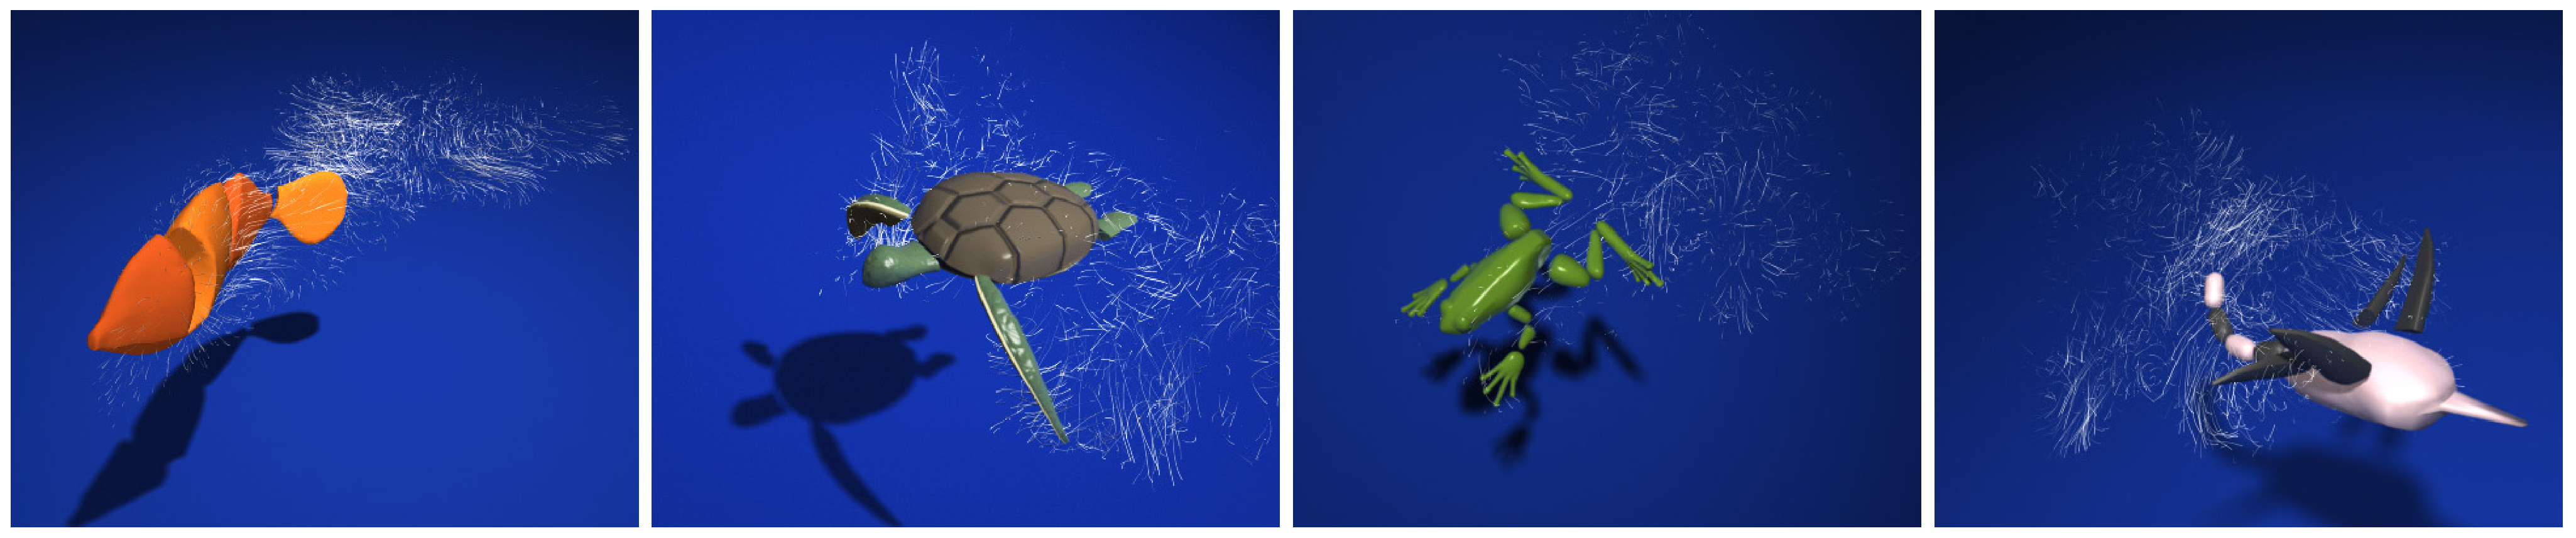
\includegraphics[width=\textwidth]{figures/teaserSwimming.eps}
  \caption{Aquatic creatures swim in a physically simulated hydrodynamic environment.}
  \label{fig:teaser1}
\end{figure}

The oceans cover over seventy percent of the area on our planet. They contain a wide variety of creatures that use swimming as their primary form of locomotion. Scientific studies show that the swimming gaits of the aquatic creatures are highly efficient compared to the man-made underwater vehicles. Studying their swimming motions could help us discover better propulsion mechanisms and design more efficient undersea vehicles to explore the largest uncharted territory on our planet. In Chapter 3, we apply numerical optimization to automatically discover the most energy efficient swimming gaits for given aquatic creatures in a physically-simulated hydrodynamic environment.

A main challenge in physical simulation is to model the complex interaction between two different types of dynamic systems, such as the two-way coupling between the fluid and a swimmer represented as an articulated rigid body system. We present an accurate physical simulator \cite{} that simultaneously solves the Navier-Stokes equations for fluids, the Lagrangian dynamics for an articulated rigid body and matches their accelerations at fluid-solid boundaries. The simulation results of swimming fish and eels show vortex trails that are in agreement with laboratory measurements.

Simulating fluid itself is hard; optimizing locomotion in a hydrodynamic environment is even more challenging. Previous methods have resorted to simplified fluid models. However, studies have shown that fish takes advantage of surrounding vortices, which are omitted in the simplified models, to provide energy boosts. Incorporating an accurate Navier-Stokes fluid model in the simulation presents new challenges in controller optimization: The optimization space is full of local minima due to the chaotic fluid behavior. Evaluating the gradient of the objective function is time-consuming. We demonstrate that sampling-based optimization algorithms are effective tools to overcome these challenges. This approach found efficient swimming motions that are comparable to those of real-world animals (Figure \ref{fig:teaser1}). 

\subsection{Locomotion for Soft Body Characters}

\begin{figure}[!h]
  \centering
    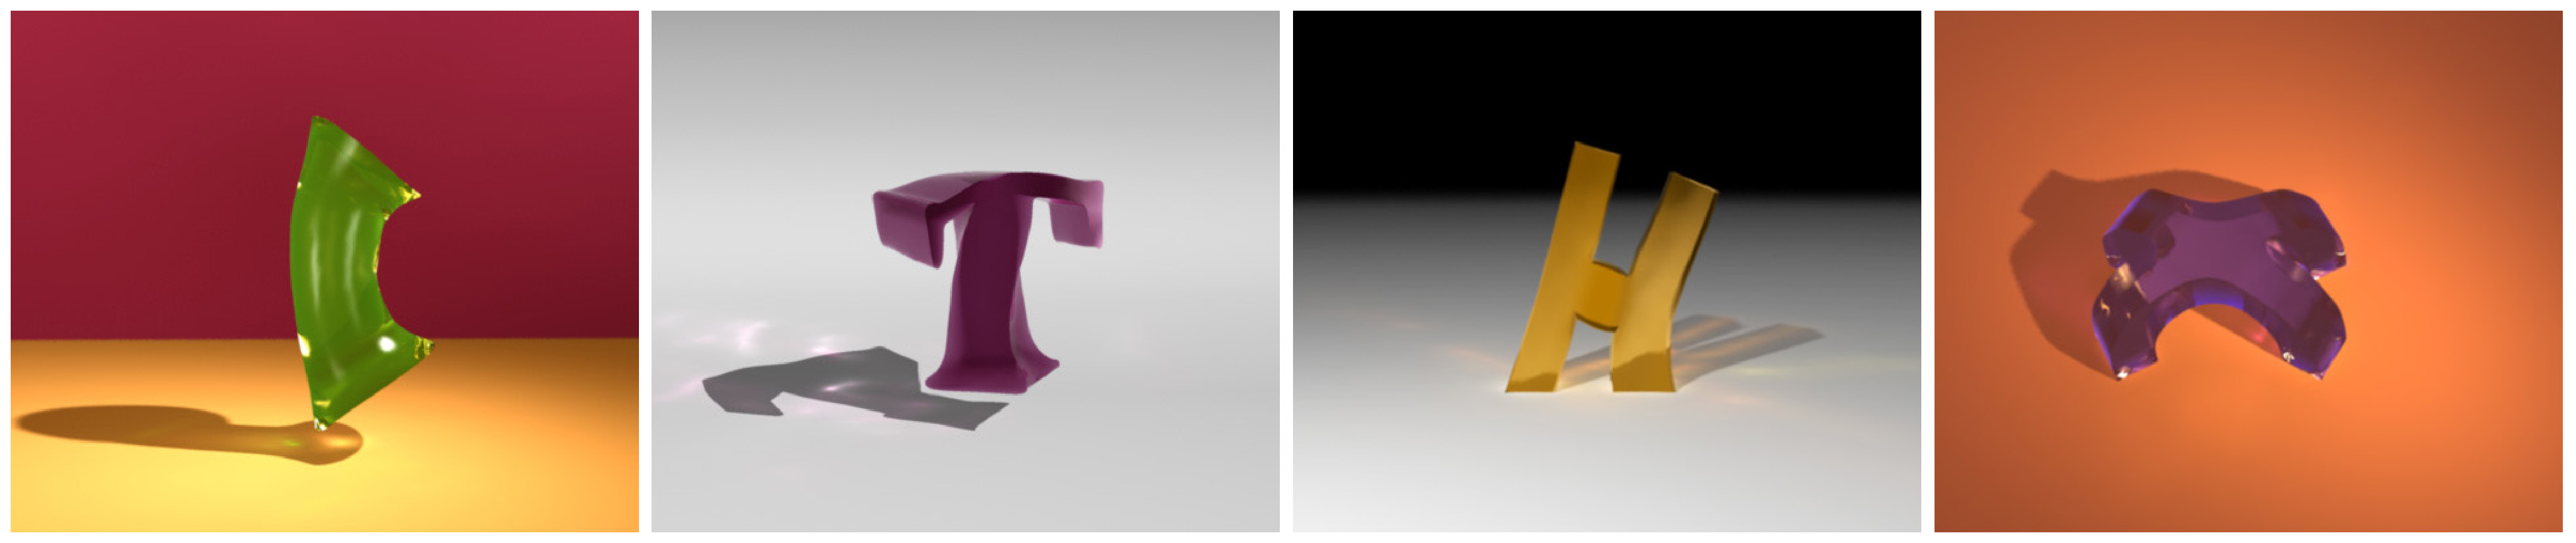
\includegraphics[width=\textwidth]{figures/teaserSoftBody.eps}
  \caption{Soft body characters perform different forms of locomotion.}
  \label{fig:teaser2}
\end{figure}

While most research in character animation and robotics focus on characters that are made exclusively from rigid parts, we have seen an increasingly amount of efforts in the last few years to develop soft body robots \cite{}. While these research demonstrates a huge potential of soft body robots and their broad applications, it demands a new set of computational tools to study and to synthesize motions for soft body characters.

To model soft body characters, we not only need to simulate the passive dynamics of deformation, but also the actuation of muscles. In Chapter 4, we present a new mathematical model for artificial muscles that are motivated by the muscle structures of soft body animals in nature. Similar to real muscles, these artificial ones are arranged in groups and only allowed to contract. Complex movements need to be accomplished by the coordinated contraction of multiple muscle groups. We develop a finite element method with this muscle model to simulate soft body animals.

Optimizing controllers in the presence of discontinuous contact forces is a long-standing problem. Controlling locomotion for soft body characters (Figure \ref{fig:teaser2}) exacerbates the difficulty. The deformation of the body constantly changes the contact configuration between the character and the ground. A common practice is to separate contact planning and controller optimization. We identify that this simplification eliminates effective control strategies, and this causes the soft body character to lose balance. We derive an elegant solution to this problem that combines contact planning with controller optimization. We formulate a quadratic program with complementarity conditions (QPCC) and develop an efficient solver for QPCC problems derived from locomotion control with contacts. As a result, effective control strategies emerge automatically from the QPCC solution.

\subsection{Locomotion with Mechanical Devices}

\begin{figure}[!h]
  \centering
    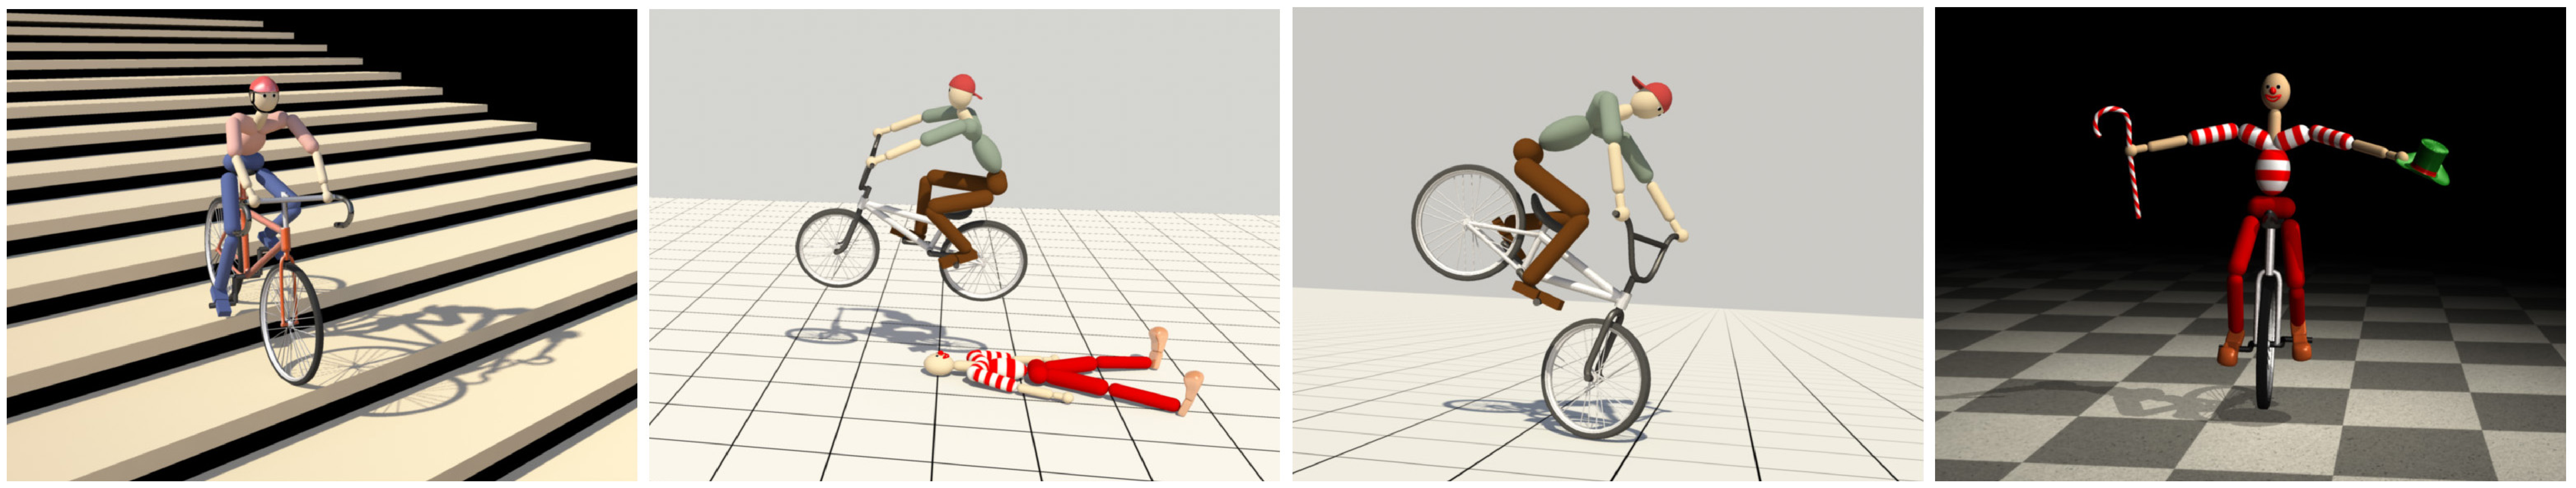
\includegraphics[width=\textwidth]{figures/teaserBicycle.eps}
  \caption{A human character performs stunts on a road bike, a BMX bike and a unicycle.}
  \label{fig:teaser3}
\end{figure}

Human has invented numerous mechanical tools to ease our life. Robots in the future can work much more efficiently if they can take advantage of these existing tools. Instead of manually programing the robots to master each tool, we hope that they can learn how to use them autonomously. Learning to ride a bicycle is an excellent case study. The bicycle, which has greatly boosted the efficiency of locomotion, was voted as the best invention since the 19th century. Even though the dynamics of bicycles is relatively well-understood, riding a bicycle is challenging due to the inherently unstable dynamics. In Chapter 5, we present a machine learning algorithm that allows a virtual character to learn to ride a bicycle in a physically simulated environment. 

In addition to the basic maneuvers, we hope that the character can learn more challenging but visually spectacular stunts (Figure \ref{fig:teaser3}). Performing stunts requires fast reaction, precise control and years of practice. This challenges the best human riders, let alone a machine learning algorithm. When we design the policy search algorithm, we find that the widely-used assumption of a predetermined controller parameterization severely limits the search space. It leaves the hard work to the user to design a good parameterization. We decide that optimizing the parameterization automatically is equally important as optimizing the parameters. Our algorithm evolves both the policy parameterization and the parameters simultaneously. This significantly improves the quality of the resulting controllers. Eventually, our simulated characters learn to perform a wide variety of bicycle stunts within hours, which is even faster than the best human stunt bikers.

\subsection{Locomotion Controller Transfer from Virtual to Real World}

Above three works demonstrate that with the powerful computational tools for character animation, natural, agile and robust motions can be synthesized efficiently and autonomously. However, creating lifelike robots is still an extremely challenging, trial-and-error process that is restricted to experts. The fast evolution of 3D printing technology will soon trigger a shift in the robotics industry from mass production to personalized design and fabrication, which will result in an immediate need for a faster, cheaper and more intuitive way to design robotic controllers. The computational tools we developed can potentially automate and streamline the process if we can transfer the controllers from the virtual simulation to the real world.

Transfering controllers optimized in a simulation onto a real robot is a non-trivial task. An optimal controller that works in a state-of-the-art simulation often fails in a real environment. This is known as the \emph{Reality Gap} \cite{}. This gap is caused by various simplifications in the simulation, including inaccurate physical model, unmodeled actuator dynamics, assumptions of perfect sensing and zero latency. In Chapter 6, we investigate some of these simplifications and present a general framework of simulation calibration. Simulation calibration optimizes simulation parameters to minimize the discrepancy between the data collected from real experiments on the robot and that generated in the simulation. After calibration, the simulation becomes more faithful to the real-world dynamics. Controllers that are designed with the improved simulator can work in both the virtual and the real world. 

\section{Contributions}

The computational tools presented in this dissertation provide several contributions to the communities of character animation and robotics. These contributions are as follows.

\paragraph{A stable simulation of two-way coupling between fluids and articulated rigid bodies.} We present a novel swimming simulator that can simultaneously solve the dynamics of fluids, articulated rigid bodies and their two-way interactions. Compared to the traditional two-way coupling solver that alternates the fluid update and the rigid body update, our method is more numerically stable. We are able to use time steps of 33ms for all our experiments without any stability problem. Using larger time steps makes our simulation orders of magnitude faster than the alternating solver. As a result, we can discover a swimming gait within days of computation while using the traditional two-way coupling technique may take weeks.

\paragraph{A finite element simulation with a muscle model for soft body animals.} Based on the muscle structure of muscular hydrostat \cite{} in real soft body animals, we develop a muscle model for the simulated characters. Combined with the finite element method for the passive deformation of the body, it provides intuitive ways to control the character in a coordinated manner. The use of this muscle model reduces the dimensionality of the control problem and results in more natural-looking motions.

\paragraph{An QPCC solver for controller optimization with changing contacts.} Controlling locomotion with contacts is a long-standing problem in continuous optimization because changes of contact situation (static, sliding or breaking) can introduce discontinuities to the dynamics. A commonly-used technique is to separate contact planning and controller optimization. However, this could eliminate effective locomotion strategies. We solve this problem by formulating a quadratic program with complimentarity conditions (QPCC). We also develop an efficient solver for QPCC problems with contacts. This method can optimize both the contact situation and forces simultaneously. As a result, interesting and effective locomotion strategies emerge automatically from the QPCC solution.

\paragraph{A reinforcement learning algorithm that searches both the parametrization and the parameters of a policy.} We present the first reinforcement learning algorithm which demonstrate that extremely challenging locomotion tasks, such as bicycle stunts, can be learned efficiently in simulation. Most of the stunt actions are learned within one hour, which is even faster than the performance of best human stunt bikers. These results present a new benchmark for future research in reinforcement learning. The key to such an efficient learning algorithm is an evolutionary optimization that can search for the parametrization and the parameters of a control policy simultaneously. We believe that this reinforcement learning algorithm can be generalized to master other challenging locomotion tasks.

